
%*****Instantaneous PSNR In relatively Bad Network Condition*****	

\begin{figure*}[!t]
	%\begin{figure*}[t]
	\centering
	\subfigure[Video Sequence 1]  {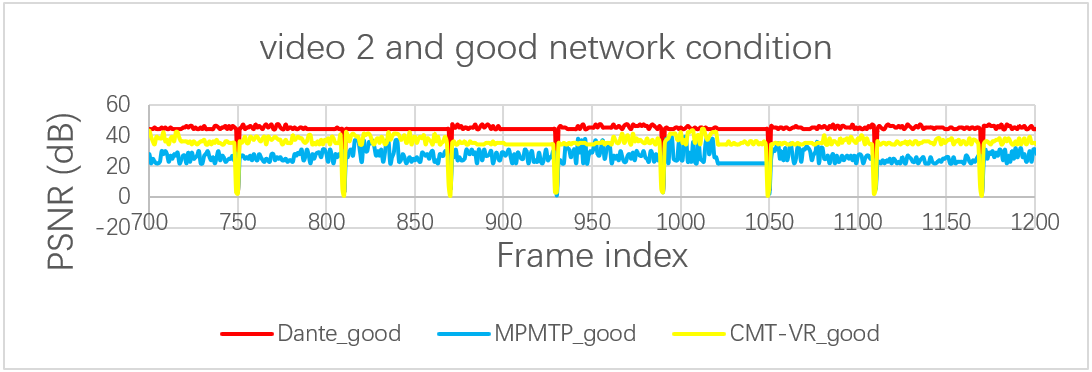
\includegraphics[scale=0.26,angle=0]{paper_figs/evaluation_result/sub/ins_psnr_v2_good.png}}
	\subfigure[Video Sequence 2]  {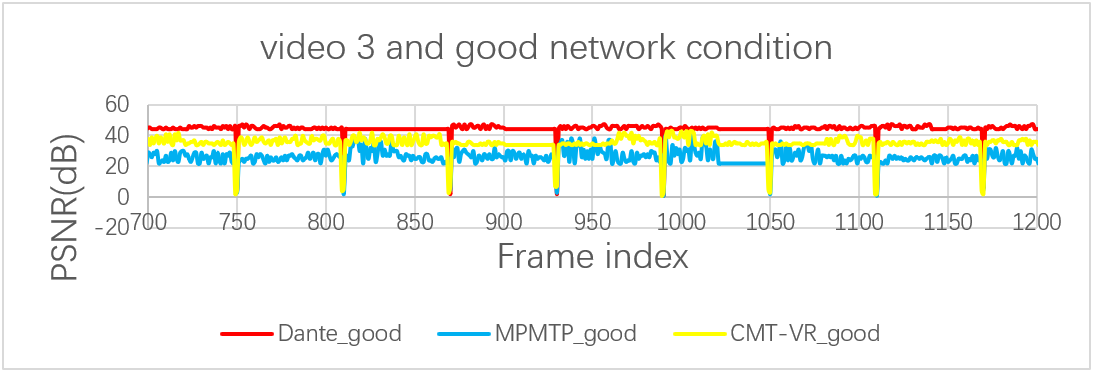
\includegraphics[scale=0.26,angle=0]{paper_figs/evaluation_result/sub/ins_psnr_v3_good.png}}
	\vspace{-0.3cm}
	\caption{Instantaneous PSNR In Relatively Good Network Condition}
	\vspace{-0.4cm}
	\label{fig:apuct}
\end{figure*}

%*****Instantaneous PSNR In relatively Good Network Condition*****
\begin{figure*}[!t]
	%\begin{figure*}[t]
	\centering
	\subfigure[Video Sequence 1]  {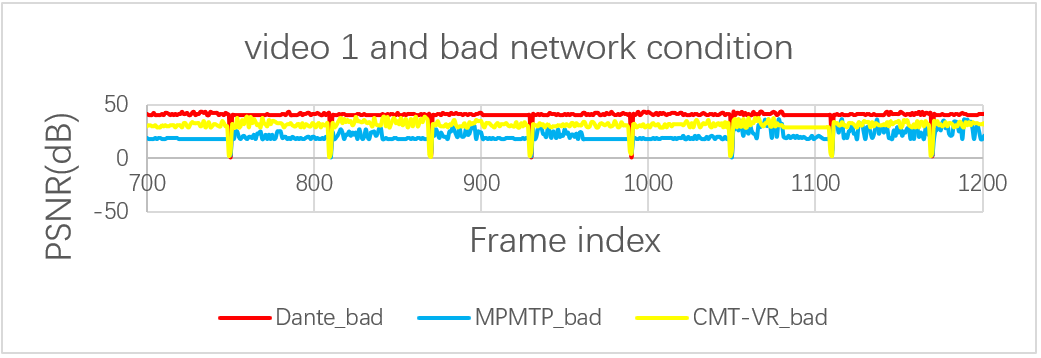
\includegraphics[scale=0.275,angle=0]{paper_figs/evaluation_result/sub/ins_psnr_v1_bad.png}}
	\subfigure[Video Sequence 2]  {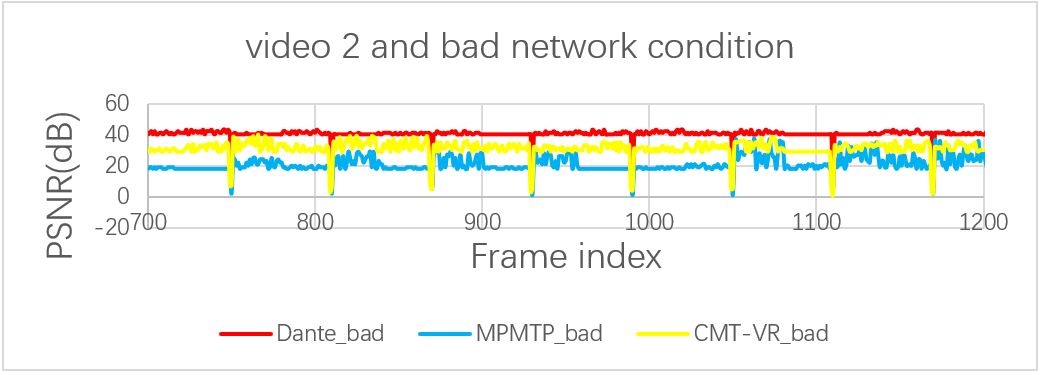
\includegraphics[scale=0.27,angle=0]{paper_figs/evaluation_result/sub/ins_psnr_v2_bad.png}}
	\vspace{-0.3cm}
	\caption{Instantaneous PSNR In Relatively Bad Network Condition}
	\vspace{-0.4cm}
	\label{fig:apuct}
\end{figure*}	




\section{Performance Evaluation}
We use PSNR as the metric of video quality and conducted extensive experiments to demonstrate Dante performance gains on video quality. 

\subsection{Reference schemes}
We evaluate the performance of Dante to compare with two video transport schemes, MPMTP~\cite{MPMTP} and CMT-VR~\cite{CMT-VR}, both of which are not FOV-aware and also utilize FEC to mitigating unnecessary retransmissions. Meanwhile, since the multi-path parallel is not our fous, so we do not take into account these two schemes' path selecting. 
\begin{packeditemize}

\item {\em MPMTP\cite{MPMTP}:} .
This video protocol utilizes the FEC to recover the data,  completely abandoning the retransmission,  in order to maximize the received data rate to prevent playback buffer starvation. This scheme performs in a video content-agnostic fashion. 

% high bandwidth
\item {\em CMT-VR\cite{CMT-VR}:}
CMT-VR, based on SCTP, utilize a quality-driven FEC redundancy  allocation to minimize the distortion of each GOP. Raptor code used to mitigate retransmission. While this scheme considers frame priority, \ie I, P frames, it is in a non-FOV-aware fashion. 

\end{packeditemize}


\subsection{Experimental Set-up}
\textbf{Experiment topology:} The server is connected with the client through one lossy links and Dante is deployed on both server and client side. The topology is not shown because of space limitation. The experiment scenario is that sources send the data to sinks through one lossy links with the request of video data.

\textbf{Testbed configuration:} The sources and sinks are commodity servers with Ubuntu 16.4 (kernel 4.40), each of which is equipped with an Intel(R) Core(TM) i3-4150k cpu @ 3.5GHz (4 cores), one Intel 82599ES 10G dual port NICs and 32 G memory.

\textbf{Parameter sets}
Timeout for triggering I frames' retransmission, $T_I$, is set to 200ms, the size of GOP is set to 15 and the length of video segment, which is request by users each time, is sent to 1s, equal to the time of 2 GOPs. Meanwhile, the size of the receiver buffer is set to 100Mb.
We evaluate the quality of video by computing the expected value of PSNR. So, given a video segment, it's PSNR can be calculated via: \[{V_{PSNR}} = \sum\limits_{i = 1}^{{\Omega ^\alpha }} {({\gamma ^\alpha } \cdot V_{PSNR}^{^\alpha })} \]
where, ${V_{PSNR}^{^\alpha }}$ is the PSNR of the layer $\alpha$. According to a tiles viewing probabilities \cite{360ProbDASH} and (Eq. 7), $\gamma ^\alpha$ can be approximately obtained and $\gamma ^\alpha$ of FOV layer, cushion layer and outmost layer is almost 0.6, 0.3, 0.1, respectively.

\textbf{Network parameter set:} Gilbert model is adopted to mimic the packet loss pattern in real wireless networks, supported by traffic control (TC)~\cite{TC}, in which four parameters($\xi _i^G$, $\xi _i^B$, 1-h and 1-k) are needed, $\xi _i^G$ and $\xi _i^B$ are transition probabilities between the bad and good state, 1-h and 1-k is the loss probability in the bad state and good state, respectively. In our testbed, 1-h and 1-k are set as 1 and 0, respectively. Meanwhile, average packet loss rate is equal to $\pi _i^B = \xi _i^B/(\xi _i^B\\ + \xi _i^P)$. And the bandwidth is also set by TC. The detailed Parameter set is seen in Table 2. 

\begin{table}
	\centering 
	\scriptsize
	\begin{tabular}{cp{1.0cm}p{1.6cm}p{0.8cm}p{2.3cm}}
		\rowcolor[gray]{0.9} 
		\hline
		(A)  &  Time(Sec.)    & Bandwidth(Mbps)       &  RTT(ms) &  Average Pakcet loss rate(\%) \\

		
		&  0${\sim}$60   &  30         &    50    &  0.5 \\

		\hline
		\rowcolor[gray]{0.9}
		\hline
		(B)  &   Time(Sec.)   & Bandwidth(Mbps)       &  RTT(ms) &     Average Pakcet loss rate(\%)  \\
		
		&  0${\sim}$60   &  20         &    50    &  2.5\\
		
		\hline
		
	\end{tabular}
	\caption{Network Condition of Two Wireless networks: (A)Relatively Good Wireless Conditions And (B)Relatively Bad Wireless Conditions}
	\label{}
\end{table}
`
\subsection{Performance Comparison With Existing Protocols}

Then, Figure 5 and Figure 6 compare instantaneous PSNR of three video sequences in good network condition and bad network condition, respectively. The result shows that Dante achieves 20\% to 30\% 360-degree video PSNR performance gain, compared to MPMTP and CMT-VR. The reason why MPMTP performs worst in all protocols is that, despite no involving retransmissions and maximizing the throughput, it doesn't consider video's inherent feature, such as decoding dependencies of video codec, which should have give different frame unequal attention, and thus can't utilize effectively the network allocation to boost video quality. Meanwhile, CMT-VR performs better than MPMTP, due to its consideration of frame priority. However, unfortunately, non-FOV-aware reliability scheme makes it waste valuable bandwidth on trivial data, thus CMT-VR is the secondary one. Dante takes into account not only traditional video features aforementioned, but FOV. Benefiting from the hierarchical protection spatially and temporally, Dante achieves desirable upgrade in instantaneous PSNR. Meanwhile, we find, compared to TCP without FEC, the average CPU time of Dante's, due to the introduction of FEC computing overhead, increases from 14\% to 25\% for the sender side, and from 14\% to 26\% for the receiver side. The overhead of FEC can be ignored considering the performance gain Dante achieves.      